% Interaction nets
% Author: Marc de Falco
\documentclass[tikz,border=10pt]{standalone}
\usepackage[fancy,color=orange]{tikz-inet}
\usepackage{verbatim}

\begin{comment}
:Title: Interaction nets
:Tags: Diagrams, Macro packages
:Grid: 2x2

These examples are from the documentation of the `tikz-inet package`_ available
on CTAN. The package helps you to draw interaction nets (a graphical 
programming paradigm close to functional programming and linear logic).

.. _tikz-inet package: http://www.ctan.org/tex-archive/help/Catalogue/entries/tikz-inet.html

:Author: Marc de Falco
:Source: The `tikz-inet documentation`_

.. _tikz-inet documentation: http://www.ctan.org/tex-archive/graphics/pgf/contrib/tikz-inet/tikz-inet-doc.pdf 

\end{comment}

\begin{document}

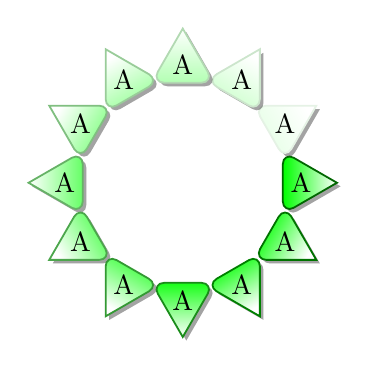
\begin{tikzpicture}
\newcount\angle
    \foreach \x in {1,...,12} {
        \pgfmathsetcount{\angle}{360*\x/12+90}
        \inetcell[\inetcellstyle=green!\x0,
            at=(\the\angle-90:1.5cm)]
            (c\x){A}[\angle]
    }
\end{tikzpicture}

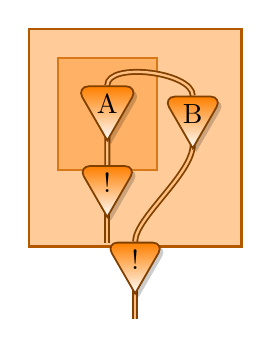
\begin{tikzpicture}
    \inetcell{A}
    \inetprombox{(A)}(pa)
    \inetcell[at=(bpa.east),right=5pt]{B}
    \inetwire(B.middle pax)(A.middle pax)
    \inetprombox{(bpa)(pa)(B)}(p)
    \inetwire(A.pal)(pa.middle pax)
    \inetwirefree(pa.pal)
    \inetwirefree(p.pal)
    \inetwire(B.pal)(p.middle pax)
\end{tikzpicture}

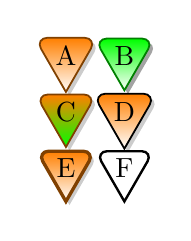
\begin{tikzpicture}
\matrix{
    \inetcell{A} &
    \inetcell[fancycellstyle=green]{B} \\
    \inetcell[bottom color=green]{C} &
    \inetcell[draw=black]{D} \\
    \inetcell[very thick]{E} &
    \inetnofancy \inetcell{F} \inetfancy \\
};
\end{tikzpicture}

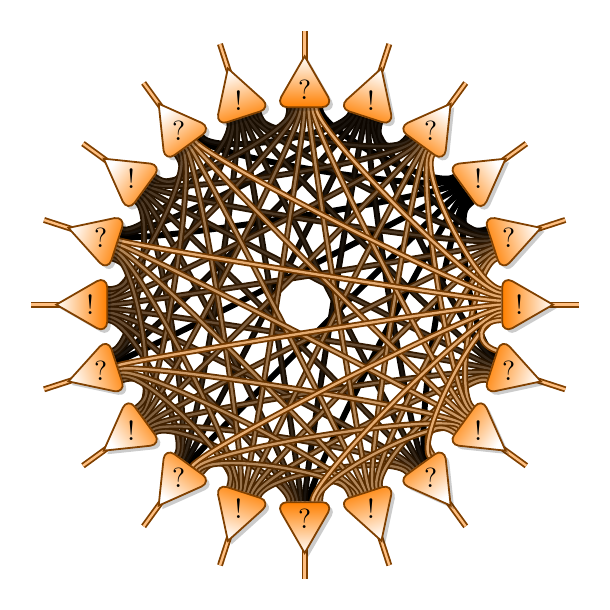
\begin{tikzpicture}
\newcount\angle
    \newcount\order
    \order=10
    \newcount\arity
    \pgfmathsetcount{\arity}{\order-1}
    \foreach \x in {1,...,\order} {
        \foreach \y/\symbol in {0/!,1/?} {
            \pgfmathsetcount{\angle}
                {(180*(2*\x+\y))/\order+90}
            \inetcell[at=(\the\angle-90:\the\order*1.8ex),
                arity=\order-1](c\y\x){\symbol}[\angle]
            \inetwirefree(c\y\x.pal)
        }
    }

    \newcount\nextcell
    \newcount\nextport
    \newcount\depth
    \foreach \x in {1,...,\order} {
        \foreach \y in {1,...,\arity} {
            \pgfmathsetcount{\nextcell}
                {mod(\x+\y-1,\order)+1}
            \pgfmathsetcount{\nextport}
                {\arity-\y+1}
            \pgfmathsetcount{\depth}{(\x-1)*100/\order}
            \inetwire[\inetwirestyle=\inetcolor!\the\depth!black]%
                (c0\x.pax \y)(c1\the\nextcell.pax \the\nextport)
        }
    }
\end{tikzpicture}
\end{document}
